\documentclass[english,phd]{diploma}

% Packages
\usepackage[autostyle=true]{csquotes} % enhanced support for quotation marks, support for biblatex package
\usepackage[backend=biber, style=iso-numeric, alldates=iso, maxbibnames=3]{biblatex}
\usepackage{dcolumn} % numeric column type
\usepackage{subfig} % subtables and subfigures
\usepackage[cpp]{diplomalst}
\usepackage{hyperref}
\usepackage{todonotes}
\usepackage{tikz}
\usetikzlibrary{graphs}
\usetikzlibrary{positioning}
\usetikzlibrary{arrows.meta}
\usetikzlibrary{math}

% Fix arrow tips
\tikzset{tips=proper}

% Commands
\newcommand{\comment}[1]{}

% Tools
\newcommand{\estee}{\emph{Estee}}
\newcommand{\rsds}{\emph{RSDS}}
\newcommand{\hyperqueue}{\emph{HyperQueue}}
\newcommand{\dask}{\emph{Dask}}
\newcommand{\ray}{\emph{Ray}}
\newcommand{\snakemake}{\emph{SnakeMake}}

% TikZ styles
\tikzset{%
    task/.style={circle, draw},
    data/.style={rectangle, draw, rounded corners},
    arrow/.style={draw, thick, {->}}
}

% Metadata
\ThesisAuthor{Ing. Jakub Beránek}

\ThesisSupervisor{Ing. Jan Martinovič, Ph.D.}

\CzechThesisTitle{Ergonomie a efektivita workflow na HPC klastrech}
\EnglishThesisTitle{Ergonomics and efficiency of workflows on HPC clusters}

\SubmissionYear{2023}

\Acknowledgement{I would like to thank all those who helped me with the work, because without
them this work would not have happened.}

\CzechAbstract{TODO}
\CzechKeywords{distribuované výpočty, výpočetní grafy, vysokovýkonnostní počítání}

\EnglishAbstract{TODO}
\EnglishKeywords{distributed computing, task workflows, hpc}

\addbibresource{references.bib}
\addbibresource{publications.bib}

\begin{document}
\MakeTitlePages

\listoffigures
\clearpage

\listoftables
\clearpage

\chapter{Introduction}
\label{ch:Introduction}
\gls{hpc} infrastructures are crucial for the advancement of scientific
research, as they offer unparalleled computational power that can be leveraged to perform the most
complex scientific experiments. The performance offered by \gls{hpc} clusters is
crucial (among other use-cases) in various scientific areas, such as weather
forecasting~\cite{wrf}, computational fluid dynamics~\cite{cfd},
bioinformatics~\cite{bioinformatics} or deep learning~\cite{hpcdl}.

Over the last several decades, the performance of \gls{hpc} clusters has been steadily
increasing, effectively doubling every few years, in line with Moore's Law and Dennard
scaling~\cite{mooreslaw}. However, it also became more difficult for \gls{hpc}
users to tap into that performance increase. Thirty years ago, it was possible to get essentially
double the performance for free, just by using a new (super)computer every two years, without
having to modify existing programs. This phenomenon has started to diminish by the end of the last
century, as chip designers became limited by the memory wall~\cite{memorywall} and especially
the power wall~\cite{powerwall}.

To keep up with the expectations of exponential performance increases, \glspl{cpu} had
to become more complex. Processor manufacturers started implementing various buffers and caches,
multiple cores, simultaneous multithreading, out-of-order execution and a plethora of other
techniques that would allow the \gls{cpu} to run faster, without requiring massive
increases of power draw or memory bandwidth. The existence of multiple cores and sockets and the
need for ever-increasing memory sizes has also made the memory system more complex, with
\gls{numa} memories becoming commonplace in \gls{hpc}. To achieve even
more performance, \gls{hpc} clusters started massively adopting various accelerators,
like the Intel Xeon Phi~\cite{xeonphi} manycore coprocessor or general-purpose
NVIDIA or AMD \glspl{gpu}, which eventually became the backbone of the majority of
current supercomputers~\cite{top500gpu}. Some clusters have also adapted more unconventional
accelerators, like reconfigurable hardware, such as \glspl{fpga}, or
\gls{ai} accelerators, such as \glspl{tpu}. This trend gave rise to
heterogeneous clusters that offer various types of hardware, each designed for specific workloads.

These hardware improvements have managed to keep up with Moore's Law, but no longer without
requiring changes to the software. The increasing complexity and heterogeneity of
\gls{hpc} hardware has caused the ``\gls{hpc} software stack'' and the
corresponding programming models to become more complex, making it far from trivial to leverage the
available performance offered by supercomputers. Individual computers of \gls{hpc}
clusters (called \emph{computing nodes}) can consist of hundreds of \gls{cpu} cores
each, yet it is quite challenging to write programs that can scale to such high core counts. The
\gls{ram} of each node contains multiple levels of complex cache
hierarchies, and it has such a large capacity that it has to be split into multiple physical
locations with varying access latencies (\gls{numa}), which requires usage of
specialized programming techniques to achieve optimal performance. And the ever-present
accelerators, for example \glspl{gpu}, might require their users to adopt completely
different programming models and frameworks.

Historically, optimized \gls{hpc} software was usually written using system or
scientifically focused programming languages (e.g.~\texttt{C}, \texttt{C++}
or \texttt{Fortran}) and specialized libraries for parallelizing and distributing
computation, such as \gls{openmp}~\cite{openmp}, CUDA~\cite{cuda} or
\gls{mpi}~\cite{mpistudy}. While these rather low-level technologies are able
to provide the best possible performance, it can be quite challenging and slow to develop (and
maintain) applications that use them. It is unreasonable to expect that most domain scientists that
develop software for \gls{hpc} clusters (who are often not primarily software
developers) will be able to use all these technologies in an efficient manner without making the
development process slow and cumbersome. This task should be left to specialized performance
engineers, enabling the scientists to focus on the problem domain~\cite{dace}.

With the advent of more powerful hardware, \gls{hpc} systems are able to solve new
problems, which are more and more demanding, both in terms of the required computational power, but
also in terms of data management, network communication patterns and general software design and
architecture. Areas such as weather prediction, machine learning model training or big data
analysis require executing thousands or even millions of simulations and experiments. These
experiments can be quite complex, consisting of multiple dependent steps, such as data ingestion,
preprocessing, computation, postprocessing, visualization, etc. It is thus imperative for
scientists to have a quick way of prototyping these applications, otherwise their development
process would be too slow.

The growing complexity of \gls{hpc} hardware, software and use-cases gave rise to the
popularity of (distributed) task-based programming models and paradigms. Task-oriented programming
models allow users to focus on their problem domain and quickly prototype, while still being able
to describe complicated computations with a large number of individual steps and to efficiently
utilize the available computational resources. Using a task-based approach, a computational
workflow is described using a set of atomic computational blocks (\emph{tasks}) that are
composed together in a \emph{task graph} which captures dependencies between the individual
tasks. Task graphs abstract away most of the complexity of network communication and
parallelization, and they are general enough to describe a large set of programs in a practical and
simple way. At the same time, they remain amenable to compiler-driven optimization and automatic
parallelization, which helps to bring the performance of programs described by a task graph close
to manually parallelized and distributed programs, at a fraction of the development cost for the
application developer. They are also quite portable, as the task graph programming model typically
does not make many assumptions about the target platform, therefore the same task graph can be
executed on various systems and clusters, provided there is a task execution runtime implemented
for that cluster.

Combined with the fact that task-based tools often allow users to implement their workflow in very
high-level languages, such as Python, or various \glspl{dsl}, it makes them an ideal
tool for rapid scientific prototyping.

Task graphs are already commonly being used and deployed on various distributed
systems~\cite{pegasus, workflows_at_scale, large_scale_modelling}, yet there are certain challenges that limit their usage ergonomics
and performance efficiency when deployed specifically on \gls{hpc} systems. These
challenges stem from various factors, such as the interaction of task graphs with
\gls{hpc} allocation managers, the heterogeneity and complexity of
\gls{hpc} cluster hardware, or simply from the potentially enormous computational
scale. When task graph authors encounter these problems, they might have to step out of the comfort
zone of this easy-to-use programming model, and implement parts of their applications using other,
more complicated approaches, to either meet their performance goals or to even make it possible to
execute their application on \gls{hpc} clusters at all. Removing or alleviating some
of those challenges could lower the barrier of entry, make task graph execution better suited for
various \gls{hpc} use-cases and turn it into an actual first-class citizen in the
world of supercomputing\@.

This thesis sets out to identify and analyse the existing challenges and bottlenecks, and design
approaches to alleviate them, in order to improve the execution of task graphs on
\gls{hpc} systems in two main areas, namely usage ergonomics and efficient hardware
utilization. It aims to achieve this objective via the following contributions: It introduces a
task graph simulator for evaluating the quality of task schedulers under various conditions, and
provides an extensive evaluation of several scheduling algorithms using this simulator. It provides
an analysis of the performance bottlenecks of a state-of-the-art task runtime
\dask{}, and introduces an alternative implementation of its server that provides
significant performance improvements in \gls{hpc} scenarios, while retaining backwards
compatibility. And primarily, it proposes an approach for effortless execution of task graphs in
the presence of \gls{hpc} allocation managers, and provides an implementation of this
approach in \hyperqueue{}, an \gls{hpc}-tailored task runtime that enables
ergonomic execution of task graphs on heterogeneous supercomputers with a focus on efficient usage
of hardware resources.

The thesis is structured as follows. \Autoref{ch:distributed-computing} describes various approaches for
designing parallelized programs on distributed clusters, introduces the task-based programming
model, and discusses various ergonomic challenges and performance bottlenecks of executing task
graphs on \gls{hpc} systems. \Autoref{ch:taskgraphs} then describes the task-based
programming model in detail by defining key terms related to tasks and task graphs. The two
subsequent chapters primarily focus on the performance aspects of task graph execution.
\Autoref{ch:estee} evaluates the performance of various task scheduling algorithms and
introduces \estee{}, a task graph execution simulator. \Autoref{ch:rsds} then
analyses the runtime performance of \dask{}, a state-of-the-art task runtime, and
proposes an alternative implementation of its server that is able to outperform it in various
\gls{hpc} use-cases. \Autoref{ch:hyperqueue} focuses on improving both the ergonomics
and performance aspects of task execution in the presence of \gls{hpc} allocation
managers, using a meta-scheduling design implemented by the \hyperqueue{} task runtime.
Finally,~\Autoref{ch:conclusion} summarizes the thesis and outlines future work.

%\begin{figure}
%	\centering
%	\begin{tikzpicture}[>=latex,line join=bevel,every text node part/.style={align=center}]
%		\tikzset {chapter/.style={rectangle, draw, minimum width=5cm, font=\footnotesize}}
%
%		\newcommand{\chname}[1]{\emph{\nameref{#1}}}
%		\newcommand{\chnum}[1]{\Autoref{#1}}
%
%		\node (distributed-computing) [chapter]
%		{\chname{ch:distributed-computing} \\\chnum{ch:distributed-computing}};
%
%		\node (taskgraphs) [chapter, below=of distributed-computing]
%		{\chname{ch:taskgraphs} \\\chnum{ch:taskgraphs}};
%
%		\node (estee) [chapter, below=of taskgraphs, xshift=3cm]
%		{\chname{ch:estee} \\\chnum{ch:estee}};
%
%		\node (challenges) [chapter, below=of taskgraphs,left=of estee, yshift=-1cm]
%		{\chname{ch:challenges} \\\chnum{ch:challenges}};
%
%		\node (rsds) [chapter, below=of estee]
%		{\chname{ch:rsds} \\\chnum{ch:rsds}};
%
%		\node (hq) [chapter, below=of rsds, xshift=-3cm]
%		{\chname{ch:hyperqueue} \\\chnum{ch:hyperqueue}};
%
%		\draw [->] (distributed-computing.south) -- (taskgraphs.north);
%		\draw [->] (taskgraphs.south) -- (challenges.north);
%		\draw [->] (challenges.south) -- (hq.north);
%		\draw [->] (taskgraphs.south) -- (estee.north);
%		\draw [->] (estee.south) -- (rsds.north);
%		\draw [->] (rsds.south) -- (hq.north);
%	\end{tikzpicture}
%	\caption{Diagram of the thesis chapters}
%	\label{fig:thesis-chapter-diagram}
%\end{figure}


\chapter{Task-based programming model}
\label{ch:taskgraphs}
There are many ways to design and program distributed and parallel programs for HPC clusters.
Historically, a popular way of creating HPC applications was to implement the parallelization of
computation and the distribution of data explicitly, typically using message-passing (e.g.\
MPI\footnote{Message Passing Interface}~\cite{mpi}), global address space (e.g.\
PGAS\footnote{Partitioned global address space}~\cite{pgas}) and/or multithreading (e.g.\
OpenMP\footnote{Open Multi-Processing}~\cite{openmp}) frameworks, which are designed and fine-tuned
for HPC use-cases. With an explicitly parallel program, users have a lot of control over the
exchange of data and communication between individual cores and distributed nodes, which allows
them to create very performant programs. This approach is also quite flexible and enables
expressing arbitrarily complex parallelization and data distribution strategies.

However, even though such explicitly parallelized programs can be incredibly efficient,
implementing them is notoriously difficult. Deadlocks and race conditions, which are already
problematic for multithreaded programs, are even more of an issue for distributed programs. HPC
applications that use libraries for explicit distribution of data (such as various MPI
implementations) are also typically implemented in languages such as \texttt{C} or
\texttt{C++} that are infamous for making it difficult to write correct, memory-safe
programs without memory errors and undefined behaviour. This further increases the difficulty and
decreases the speed of developing correct distributed programs.

It would be unreasonable to expect that all scientists that want to leverage HPC to execute their
experiments will ``roll up their sleeves'' and spend months implementing an explicitly parallel
\texttt{C++} program that uses MPI. A more typical scenario is that scientists leverage
existing coarse-grained tools and frameworks that are optimized for HPC and use technologies like
MPI or OpenMP internally (e.g.\ GROMACS~\cite{gromacs}). However, with both the experiments
and HPC clusters becoming ever more complex each year, it is usually not sufficient to use only a
single tool. Scientific experiments require running many independent steps, which encompass data
transfer, preprocessing, postprocessing and the usage of potentially many different tools that have
to be combined. These experiments can also be executed in potentially many instances that have
different input parametrizations.

That is why in recent years, it became popular to define scientific computations using programming
models where the high-level communication and parallelization structure of the computation is
derived automatically from the program description. There are multiple ways of achieving that, such
as using e.g.\ the MapReduce~\cite{mapreduce} model, however this thesis focuses on one
approach in particular -- scientific workflows, also called pipelines. Workflows can describe a
complex computation composed of potentially many different tool invocations that can depend on one
another. They are often written in very high-level languages, such as Python, which allows users to
focus on defining the computation easily and also to quickly prototype. Crucially, these workflows
are typically based on a programming model that does not require explicit implementation of data
exchange and parallelism -- the task-based programming model.

The task-based programming model allows users to describe the high-level structure of the
computations that they want to perform using a \emph{task graph}. Users create the task graph
by splitting their desired computation into a set of \emph{tasks}, atomic and independent
computational blocks with explicitly described inputs and outputs that can be executed in a
self-contained way. Additional constraints can also be encoded into the task graph, e.g.\ which
data should be transferred between the individual tasks, which tasks cannot be executed until some
other task finishes its execution, or the necessary properties of an environment in which a task
will be executed.

The primary benefit of describing a computational workflow in such a way is that the resulting
program is \emph{implicitly parallel}. The author of the program does not imperatively specify how
should the computation be parallelized or when and how should data be exchanged. They merely
declaratively describe the individual parts of the program that can theoretically be executed in
parallel (the tasks) and then pass the task graph to a dedicated execution tool that executes the
tasks on a parallel machine (or even on a distributed cluster). Since the program is represented
with an explicit graph, the execution tool can effectively analyze its properties (or even optimize
the structure of the graph) in an automated way, and extract the available parallelism from it
without requiring the user to define parallelization opportunities explicitly.

Note that from the perspective of a task execution tool, each task is an opaque element. The tool
knows how to execute it, but it typically does not have any further knowledge of the inner
structure of the task. Therefore, the only parallelization opportunities that can be extracted by
the tool have to be expressed by the structure of the task graph. A task graph containing a single
task is thus not very useful on its own.

The task-based programming model is central to the topic of this thesis, and thus this chapter will
define various terms and concepts related to it. Note that there are many variations of this
programming model, based on the specific tool or environment where it is used, and thus the term
\emph{task-based programming} is heavily overloaded. It is used in various related technologies, ranging
from fine-grained tasks that execute a single function or just a handful of
instructions~\cite{starpu,openmp} to coarse-grained task workflows that execute binaries which
can run for hours or even days~\cite{dask, snakemake, nextflow}. This thesis primarily focuses on the latter
type of task graphs, which represent very general computations (either functions or binaries) with
various levels of granularity, that are intended to be distributed among multiple nodes of a
distributed cluster. A further distinction can be made between batch-oriented workflows, which
define a computation with a clearly delimited set of inputs that is already available when the
workflow starts, and which focus primarily on throughput, and streaming-oriented workflows, which
operate continuously on streams of input data that arrive just-in-time, and which usually focus on
latency. This thesis focuses exclusively on batch workflows, which are more common in HPC
scenarios\todo{cite}.

The term \emph{task} is also heavily overloaded in various areas of computer science, as
it is used for many unrelated concepts, from an execution context in the Linux operating system,
through a block of code executed by the OpenMP library, to a program executed by a complex
distributed computational workflow. Even in the area of distributed computing, the terminology can
vastly differ between different task execution tools and theoretical works.

Even though task-related terms can have a lot of different meanings, depending on the context, and
an attempt of providing a single unifying task theory would need to gloss over many important
details, it is still useful to provide a shared vocabulary of terms for this thesis. This chapter
thus defines several task-related terms in a way that allows capturing the specifics of task
execution in HPC environments, further described in Chapter~\ref{ch:challenges}, and that is
general enough so that it can be mapped to concepts used by task execution tools that will be
described in later chapters.

\section{Task graph}
A computational workflow in the task-based programming model is represented with a directed acyclic
graph (DAG) that we will label as a \emph{task graph}. From a high-level perspective, it
describes which individual steps should be performed, what are the constraints for where and in
which order are they computed and how should data be transferred between the individual steps of
the workflow.

There are many variations of task graphs, based on the computational properties that they are able
to describe. In the most basic form, task graph vertices represent computations to be performed,
and the edges represent dependencies between the computations, which enforce an order in which will
the computations be performed. However, numerous other concepts can also be encoded in a task
graph. For example, in addition to dependencies, the edges could represent abstract communication
channels, through which the outputs of one computation are transferred to become the inputs of
another computation that depends on it. There could be a special type of edge which specifies that
the outputs of a computation will be streamed to a follow-up computation, instead of being
transferred only after the previous computation has finished. There could also be e.g. a special
type of node that defines iterative computation that is performed repeatedly until some condition
is met.

The exact semantics of vertices and edges of task graphs depend heavily on the specifics of tools
that implement them, and thus it is not possible to have a single definition that would fit all
variants used ``in the wild''. To provide a general description, we will formally define a task
graph designed for batch workflows, which can capture the structure of dependencies between
computations and the notion of transferring data between them. This definition is general enough so
that it can be mapped to the task execution tools described later in this thesis.

A task graph is a tuple $(T, O, E)$, where $T$ is a set of
\emph{tasks}, $O$ is a set of \emph{data objects} and
$E \subseteq ((T\times{}O) \cup (O\times{}T))$ is a set of arcs. $(T \cup O, E)$ forms a finite directed acyclic
graph. The graph is structured in a way so that for every data object, there is exactly one task
that produces it: $\forall o\in{}O: (\exists t_1\in{}T: (t_1, o) \in E \land
	(\forall
	t_2\in{}T: (t_2, o) \in E \Rightarrow t_1 = t_2))$.

Below we will define several terms and properties that will be useful for working practically with
task graphs:
\begin{enumerate}
	\item If there is an arc between a task and a data object ($(t,o) \in (T\times{}O)$), then we call
	      $t$ the \emph{producer} of $o$ and $o$
	      the \emph{output} of $t$.
	\item If there is an arc between a data object and a task ($(o,t) \in (O\times{}T)$), then we call
	      $t$ the \emph{consumer} of $o$ and $o$
	      the \emph{input} of $t$.

	\item Let us introduce a binary relation $D_r$ over the set of tasks:
	      $\{(t_1, t_2): (t_1, t_2)\in{}(T\times{}T)\land t_1 \neq t_2 \land
		      \exists{}o\in{}O: (t_1, o)\in{}E
		      \land (o, t_2)\in{}E\}$. When $(t_1, t_2) \in D_r$, we say that $t_2$
	      \emph{directly depends} on $t_1$. We can also state that $t_2$
	      consumes the output produced by $t_1$.

	\item Let us introduce a binary relation $D$ over the set of tasks. Tasks
	      $t_1$ and $t_n$ are in this relation if there is a sequence
	      $(t_1, t_2, \ldots, t_n)$ such that $\forall i \in \{
		      1,2,\ldots,n - 1\}: (t_i, t_{i+1}) \in D_r$. When $(t_1, t_2) \in D$, we say that
	      $t_2$ \emph{depends} on $t_1$ and that
	      $t_1$ is a \emph{dependency} of $t_2$.

	\item We label tasks without any dependencies \emph{source tasks}. $S = \{ t \mid t\in{}T \land \forall{}t_d\in{}T:
		      (t_d, t)\notin D\}$. It is a
	      simple observation that unless the task graph is empty ($(T\cup{}O) = \emptyset$), there is always at
	      least one source task in the graph, because the graph is acyclic.
	\item We label tasks that are not depended upon by any other task \emph{leaf tasks}.
	      $L = \{ t \mid t\in{}T \land \forall{}t_d\in{}T: (t,
		      t_d)\notin D\}$.
\end{enumerate}

An example of a simple task graph is shown on Figure~\ref{fig:task-graph-example}. Tasks are represented
as circles, data objects as (rounded) rectangles\footnote{This representation will be used in all following task graph diagrams.} and arcs as arrows. The
source task $t_0$ generates two data objects, which are then used as inputs for
four additional tasks. The outputs of these four tasks are then aggregated by a final task
$t_5$. This can correspond e.g.\ to a workflow where $t_0$
generates some data, $t_{1-4}$ performs some calculation on that data and
$t_5$ performs some post-processing step and stores the results to disk.

\begin{figure}[h]
	\centering
	\resizebox{!}{35mm}{
	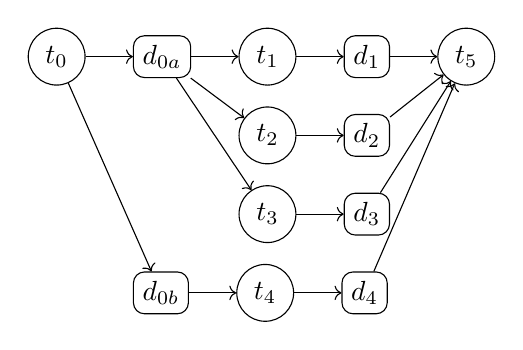
\begin{tikzpicture}
            \graph[
                grow right sep=6mm,
            ] {
                "$t_0$"[task] -> {
                    "$d_{0a}$"[data] -> {
                        "$t_1$"[task] -> "$d_{1}$"[data],
                        "$t_2$"[task] -> "$d_{2}$"[data],
                        "$t_3$"[task] -> "$d_{3}$"[data]
                    },
                    "$d_{0b}$"[data] -> {
                        "$t_4$"[task] -> "$d_{4}$"[data]
                    }
                } -> "$t_5$"[task]
            };
        \end{tikzpicture}
	}
	\caption{Simple task graph with six tasks and six data objects}
	\label{fig:task-graph-example}
\end{figure}

Note that the presented definition of a task graph does not describe its semantics -- how will the
graph be created and executed and what will be the interactions between tasks and data objects.
This depends on the specific tool or framework which uses task graphs to define its programming
model. For example, in a distributed batch oriented setting, if a task $t_2$
depends on another task $t_1$, then $t_2$ cannot start to execute
until $t_1$ has finished executing and the data objects produced by
$t_1$ have been transferred to the computational node that will execute
$t_2$.

\emph{Data object} is commonly represented as a serialized blob of data that has to be
transferred from the node where its producer was computed to the node where its consumer is to be
executed. If a task programming model does not encode any direct transfer of data between tasks,
then the data objects serve simply as ``empty'' markers of dependencies, and they do not hold any
actual data. In that case, we could even remove them from the task graph completely, and represent
direct dependencies with arcs between tasks.

\emph{Task} is a serializable description of a computation that can be executed
repeatedly. The serializability property is crucial, as it allow us to treat computations as data,
which is quite powerful, because it allows tasks to be sent between different nodes in a cluster or
stored to disk and to be transparently recomputed an arbitrary number of times. Tasks might need to
be recomputed e.g.\ after some failure occurs during their execution.

In practice, a single task will typically represent either the invocation a function (a block of
code that can be executed in a self-contained way) or the execution of a program (an executable
binary). Multiple tasks in a task graph can execute the same function or executable, and this is in
fact the common case, as task graphs are often used to parametrize a single computation with many
different input parameters.

Even though in the formal definition the inputs and outputs of tasks are sets, in practice they are
usually represented either with ordered sequences or some mapping that associates a name with each
input or output, because it is important to distinguish the identity and/or the order of each input
and output. For functions, inputs are its arguments, and output is its return value, which can be
structured so that a sequence of outputs is generated, instead of just a single output. For binary
programs, inputs are e.g.\ command-line arguments or the content of its \texttt{standard input stream}, and
the output can be e.g.\ the content of the \texttt{standard output stream} generated by the executed
program.

While inputs and outputs explicitly describe how data flows in and out of tasks, when a task is
executed, it can additionally also read the state of the environment in which it is being executed,
or change the state in a way that is observable by other tasks. For example, a function can read or
modify the value of a global variable, or an executable can read an environment variable or create
a file on a disk which is not specified as a task output. Such actions, which we will label as
\emph{side effects}, are typically not encoded within the task graph. Tasks should ideally
contain as few side effects as possible, because they can make task execution non-deterministic, by
causing it to produce different outputs when executed multiple times, which might not be desired.
To actually produce some output, most task graphs will eventually store some data to a file-system,
which can be either considered a side effect, or a first-class operation, depending on the
semantics of the task execution tool.

Apart from specifying the structure of required inputs and produced outputs, tasks can also define
various constraints for the environment in which they will be executed. We will use the term
\emph{resource requirements} for such constraints. As an example, a task that performs training of a
machine learning model might require a GPU (Graphics Processing Unit) to be present on the
computational node where the task will be executed. Other resources might include e.g.\ a minimum
required amount of memory (RAM) or a required amount of processor cores necessary to execute the
task.

\section{Task graph execution}
Task graphs merely describe some computation, therefore they have to be executed in order to
actually produce some results (outputs). This is the responsibility of a \emph{task runtime}, a
tool that analyzes task graphs and executes them in some \emph{computational environment}, e.g.\ a personal
computer or a distributed cluster. Such an environment contains a set of computational providers
that are able to execute tasks, these providers are commonly labeled as \emph{workers}. The
\emph{execution} of a task is the act of performing its described computation by a specific
worker (or a set of workers) with specific input(s), and producing some output(s).

There are many existing task runtimes, with varying architectures, features and trade-offs, which
affect factors like performance, fault tolerance or expressivity of the supported variant of the
task-based programming model. Some of these existing runtimes will be described in more detail in
Chapter~\ref{ch:sota}. We will consider a common scenario in the rest of this chapter,
which is a distributed task runtime with a centralized management component and a set of workers
that communicate with it via network or inter-process comunication.

In general, a task runtime manages and monitors all aspects of task graph execution; primarily it
manages tasks and workers. This agenda can be quite complex especially in a distributed setting,
where the workers operate on remote computational nodes connected by a network.

Worker management involves handling the lifetime of workers (their connection/disconnection),
facilitating data transfers between them or providing resiliency in case of worker failures. A
single worker is typically a program running on a computational node, which is connected to the
management component of the runtime. It receives commands from it, executes tasks and sends
information about task execution status back to it. Each worker typically manages some hardware
resources that are available for tasks during their execution. Hardware resources can be assigned
to workers in various ways. There can be a single worker per whole computational node, or there
could be multiple workers per node, each one managing a subset of the available resources (e.g.\ a
worker per CPU core).

The second main aspect that has to be handled by the runtime is the management of tasks. It has to
keep track of which tasks have already been computed, which tasks are currently being executed on
some worker(s) or which tasks are ready to be executed next because their dependencies have already
been computed. Two important responsibilities in this area are fault tolerance and scheduling.

Fault tolerance is the ability to gracefully handle task execution failures, and provide ways of
retrying failed computations. When the execution of a task fails with some error condition (e.g.\
because a worker executing the task crashes), a fault-tolerant task runtime will be able to
transparently restart it by launching a new execution of that task. We will use the term
\emph{task instance} for a specific execution of a task. Runtimes might impose some limits on
retrying failed tasks, e.g.\ by attempting to execute up to a fixed amount of task instances for
each task before giving up, to avoid endless failure loops.

Tasks are usually considered to be atomic from the perspective of the runtime, i.e.\ they either
execute completely (and successfully), or they fail, and then they have to be restarted from
scratch. Granularity thus plays an important factor here -- if a task is large, then a lot of work
might have to be redone if it fails and is re-executed. Some runtimes try to alleviate this cost by
enabling task checkpointing, which is able to save a computational state during task execution and
then restore computation from it in case of a failure, thus avoiding the need to start from the
beginning.

Fault tolerance is challenging in the presence of dependencies. When a task has inputs, the runtime
might have to store them (either in memory or in a serialized format on disk) even after the task
has started executing. Because there is always a possibility that it will have to restart the task
in case of a failure, and thus it needs to hold on to its inputs. In some cases it can be a better
trade-off to avoid storing the inputs and instead re-execute the dependencies of the task (even if
they have executed successfully before) to re-generate the inputs. This can help reduce memory
footprint, albeit at the cost of time, and it also might not work well if the dependencies are not
deterministic.

Note that the fact that we are even able to execute a task multiple times is one of the core
advantages of the task-based programming model, where tasks declaratively describe a self-contained
computation that can be re-executed arbitrarily. This crucial property of tasks makes
fault-tolerant execution of task graphs possible.

\section{Task scheduling}
Arguably the most important responsibility of a task runtime, and one that gets the most attention
in research works, is \emph{task scheduling}. It is the act of deciding in which order and on which
specific workers should each task execute, in a way that optimizes some key metric. There are many
metrics that can be optimized for, such as the latency to execute specific critical tasks, but the
most common metric is \emph{makespan} -- the duration between the start of the execution of
the first task to the completion of all tasks within the task graph. Scheduling is a crucial
activity of the runtime, as it has a profound effect on the efficiency of the whole workflow
execution. We will use the term \emph{scheduler} for a component of the task runtime that is
responsible for assigning tasks to workers.

%TODO: define what is a schedule

Figure~\ref{fig:scheduling-example} shows an example of how a schedule of a simple task graph looks like,
and how a trivial change in the schedule can severely affect the resulting makespan. The figure
contains a task graph with four tasks and two data objects. The size of the circles is proportional
to the duration of the tasks and the size of the rectangles is proportional to the size of the data
objects. Let us assume that we want to schedule this task graph to a cluster with three workers
($w_0$, $w_1$, $w_2$). Two different schedules
for this situation are shown in the figure. Schedule $S_0$ assigns tasks
$t_0$ and $t_1$ to worker $w_0$, task
$t_2$ to worker $w_1$ and task $t_3$ to worker
$w_2$. The timeline of the schedule the shows execution of tasks (gray rectangles)
and receiving of a data object from another worker (green rectangles) for each individual worker.
It is clear that with the schedule $S_1$, the task graph will be computed quicker
than with schedule $S_0$, even though the only difference between the two
schedules is the tasks $t_1$ and $t_3$ were swapped between
workers $w_0$ and $w_2$. Note that the schedule timeline assumes
that a worker can overlap the computation of a task with sending/receiving a data object, which is
a reasonable feature that is commonly provided by existing task runtimes.

\begin{figure}[h]
	\centering
	\resizebox{!}{110mm}{
	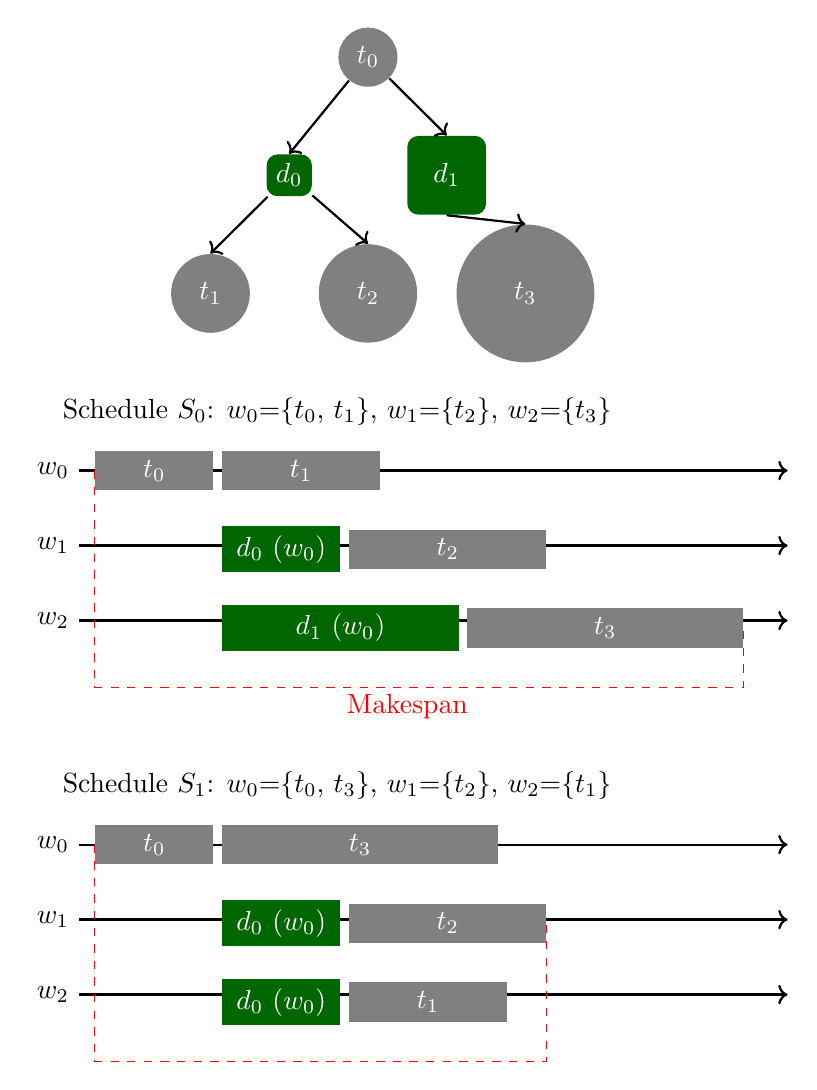
\begin{tikzpicture}
            \tikzmath{
                \tzerowidth = 15mm;
                \tonewidth = 20mm;
                \ttwowidth = 25mm;
                \tthreewidth = 35mm;
                \ozerowidth = 15mm;
                \oonewidth = 30mm;
            }
            \tikzset {
                taskstyle/.style={fill=gray, text=white, draw=none},
                objstyle/.style={fill=black!60!green, text=white, draw=none},
            }

            % T0
            \node[task, taskstyle, minimum size=7.5mm] (t0) at (0, 0.5) {$t_0$};
            \node[data, objstyle, minimum size=5mm] (d0a) at (-1, -1) {$d_0$};
            \node[data, objstyle, minimum size=10mm] (d0b) at (1, -1) {$d_1$};
            \draw [arrow] (t0) edge (d0a.north) (t0) edge (d0b.north);

            % T1 and T2
            \node[task, taskstyle, minimum size=10mm] (t1) at (-2, -2.5) {$t_1$};
            \node[task, taskstyle, minimum size=12.5mm] (t2) at (0, -2.5) {$t_2$};
            \draw [arrow] (d0a) edge (t1.north) (d0a) edge (t2.north);

            % T3
            \node[task, taskstyle, minimum size=17.5mm] (t3) at (2, -2.5) {$t_3$};
            \draw [arrow] (d0b.south) edge (t3.north);

            % Move below to draw the timelines
            \tikzset{shift={(-4,-4)}}

            \node[anchor=west] at (0, 0) {Schedule $S_0$: $w_0$=\{$t_0$, $t_1$\}, $w_1$=\{$t_2$\}, $w_2$=\{$t_3$\}};

            \tikzset{shift={(0,-0.75)}}
            \node (tim1A) at (0, 0) {$w_0$};
            \draw[arrow] (tim1A.east) -- ++(9, 0);
            \node[below = 0.5 of tim1A.south] (tim1B) {$w_1$};
            \draw[arrow] (tim1B.east) -- ++(9, 0);
            \node[below = 0.5 of tim1B.south] (tim1C) {$w_2$};
            \draw[arrow] (tim1C.east) -- ++(9, 0);

            % Timeline 1, row 1
            \node[taskstyle, minimum width=\tzerowidth, right = 0.2 of tim1A.east] (tim1t0) {$t_0$};
            \node[taskstyle, minimum width=\tonewidth, right = 0.1 of tim1t0.east] (tim1t1) {$t_1$};

            % Timeline 1, row 2
            \node[objstyle, minimum width=\ozerowidth, below = 1 of tim1t1.west, anchor=west]
            (tim1o0) {$d_0$ ($w_0$)};
            \node[taskstyle, minimum width=\ttwowidth, right = 0.1 of tim1o0.east] (tim1t2) {$t_2$};

            % Timeline 1, row 3
            \node[objstyle, minimum width=\oonewidth, below = 1 of tim1o0.west, anchor=west]
            (tim1o1) {$d_1$ ($w_0$)};
            \node[taskstyle, minimum width=\tthreewidth, right = 0.1 of tim1o1.east]
            (tim1t3) {$t_3$};

            \draw[dashed, draw=red] (tim1t0.west) -- ++(0, -2.75) --
            ([shift=({0,-0.75})]tim1t3.east) -- (tim1t3.east);

            \node[text=red] at (4.5, -3) {Makespan};

            % Move below to draw the timelines
            \tikzset{shift={(0,-4)}}

            \node[anchor=west] at (0, 0) {Schedule $S_1$: $w_0$=\{$t_0$, $t_3$\}, $w_1$=\{$t_2$\}, $w_2$=\{$t_1$\}};

            \tikzset{shift={(0,-0.75)}}
            \node (tim2A) at (0, 0) {$w_0$};
            \draw[arrow] (tim2A.east) -- ++(9, 0);
            \node[below = 0.5 of tim2A.south] (tim2B) {$w_1$};
            \draw[arrow] (tim2B.east) -- ++(9, 0);
            \node[below = 0.5 of tim2B.south] (tim2C) {$w_2$};
            \draw[arrow] (tim2C.east) -- ++(9, 0);

            % Timeline 2, row 1
            \node[taskstyle, minimum width=\tzerowidth, right = 0.2 of tim2A.east] (tim2t0) {$t_0$};
            \node[taskstyle, minimum width=\tthreewidth, right = 0.1 of tim2t0.east] (tim2t1)
            {$t_3$};

            % Timeline 2, row 2
            \node[objstyle, minimum width=\ozerowidth, below = 1 of tim2t1.west, anchor=west]
            (tim2o0) {$d_0$ ($w_0$)};
            \node[taskstyle, minimum width=\ttwowidth, right = 0.1 of tim2o0.east] (tim2t2) {$t_2$};

            % Timeline 2, row 3
            \node[objstyle, minimum width=\ozerowidth, below = 1 of tim2o0.west, anchor=west]
            (tim2o1) {$d_0$ ($w_0$)};
            \node[taskstyle, minimum width=\tonewidth, right = 0.1 of tim2o1.east] (tim2t3) {$t_1$};

            \draw[dashed, draw=red] (tim2t0.west) -- ++(0, -2.75) --
            ([shift=({0,-1.75})]tim2t2.east) -- (tim2t2.east);
        \end{tikzpicture}
	}
	\caption{Simple task graph and two different schedules}
	\label{fig:scheduling-example}
\end{figure}

Optimal scheduling of tasks to workers is NP-hard~\cite{Ullman1975}, even in the most basic
scenarios, when the exact duration of executing each task is known, and even if we do not consider
network costs of transferring data between workers. Task runtimes thus resort to various heuristics
tailored to their users' needs. Some classic task scheduling heuristics and their comparisons can
be found in~\cite{hlfet1974,kwok1998benchmarking,hagras2003static,wang2018list,estee}.

The scheduling heuristics have to take many factors into consideration when deciding on which
worker should a task execute:

\begin{description}
	\item[\textbf{Resource requirements}] The scheduler should respect all resource requirements specified by individual tasks. The runtime
		thus has to observe the (dynamically changing) available resources of each worker and schedule
		tasks accordingly to uphold their requirements. This can be challenging especially in the presence
		of complex resource requirements.
	\item[\textbf{Data transfer cost}] If the runtime operates within a distributed cluster, one of the most important scheduling aspects
		that it needs to consider is the transfer cost of data between workers over the network. All
		benefits gained by computing a task on another worker to achieve more parallelization might be lost
		if it takes too much time to send the data (task outputs) to that worker.

		The scheduler thus has to carefully balance the communication-to-computation ratio, based on the
		available network bandwidth, sizes of outputs produced by tasks and the current utilization of
		workers.
	\item[\textbf{Scheduling overhead}] The overhead of computing the scheduling decisions itself also cannot be underestimated. As already
		stated, computing an optimal solution is infeasible, but even heuristical approaches can have
		wildly different performance characteristics. Producing a lower quality schedule sooner, rather
		than a higher quality schedule later, can be sometimes beneficial, as we have demonstrated
		in~\cite{estee, rsds}.
	\item[\textbf{Memory consumption}] It is desirable to execute as many tasks in parallel on a given worker (with respect to its
		available parallelism), to speed up the completion of the whole workflow. However, the scheduler
		must also balance the amount of executing tasks according to the total memory that they consume. In
		general, it is quite hard to predict for how long will a task execute, and how much (peak) memory
		will it consume. When a task executes longer than expected, the workflow will still be computed, it
		will just take more time. But when a task uses more memory than expected, the scheduler puts many
		such tasks on a worker, and the worker then runs out of memory, the worker will probably crash. If
		this happens repeatedly, it can stall or completely stop the execution of the workflow. For these
		kinds of memory-intensive workflows, the scheduler should assign fewer tasks at the same time to a
		single worker, or reduce memory consumption in some other way, e.g.\ by keeping less cached data
		objects in worker's memory.
\end{description}


\chapter{Task graph challenges in HPC}
\label{ch:challenges}
Task-based programming is quite popular and useful, as it provides a simple way to define complex
workflows which can then be executed in a wide range of environments, ranging from consumer
laptops, through cloud deployments, to distributed HPC clusters. However, as any programming model,
it also has some disadvantages and problems. It is crucial to understand these limitations in order
to design approaches for overcoming them.

This chapter thus describes various challenges and requirements of this programing model, both in
terms of efficient and scalable execution, and in terms of the offered productivity and ergonomics.
It focuses specifically on challenges and requirements required by HPC use-cases, which introduce a
unique set of constraints stemming both from the inherent complexity of HPC software and hardware
and also from the sheer computational scale required to efficiently utilize HPC resources.

In addition to the challenges, we will also mention various desired properties and features which
should be offered by task runtimes in order to either support the mentioned requirements or to
alleviate the mentioned problems.

\section{Allocation manager}
The vast majority of HPC systems use some kind of allocation manager (such as
PBS\slash{}Torque~\cite{pbs} or Slurm~\cite{slurm}) to
facilitate submission of computations, resource management and user
accounting~\cite{slurm-schedmd}. To perform any computation through an allocation manager, the
user has to submit an \emph{allocation}\footnote{The term \emph{job} is also commonly used for the concept of HPC computational
requests. However, we will reserve this term for a different concept described later in the thesis and use the term
\emph{allocation} for HPC computational requests.}, a computational request
that states (amongst other things) how many nodes they want to allocate and what is the expected
maximum duration of their computation. The allocation is then submitted into a
\emph{queue} and starts to execute only once there are enough free computational
resources. Allocation managers are used to provide fair access to HPC resources, to avoid their
oversubscription and also to handle accounting of computation. They tend to have fairly strict
limits on the number of allocations that users can submit and the amount of nodes that they can
have reserved for their allocations at any given time.

Since users have to create computational requests through the allocation manager, and thus they
cannot simply execute their task graphs directly on an HPC cluster, a natural question arises --
how to map tasks (or task graphs) to HPC allocations in order to efficiently utilize HPC resources?
Several ways of performing this mapping are described below, however all of them come with
significant disadvantages.

\subsection*{Execute the whole task graph in a single allocation} This is the simplest case. If the
task graph does not have a large number of tasks, or if it can be executed quickly, it could be
submitted within a single allocation. This approach is quite simple for the user, since they just
execute the task graph using some task runtime in the same way as they would on a cluster without
an allocation manager or on a personal computer. The only difference is that they have to define
and submit an allocation that will bootstrap the computation.

However, since allocations are bound both by node count and time limits, this approach will only be
usable for rather small task graphs. Indeed, if the computation is short, it might not even make
sense to use an HPC cluster to compute it. A more realistic scenario is that even if an individual
task graph can be executed quickly, users might want to execute many such task graphs (for example
to execute many experiments with different parametrizations). This situation can be seen as a
special case of a large task graph that consists of many disjoint components (smaller task
subgraphs). In this case, it will typically not be possible to execute all such task graphs inside
a single allocation.

\subsection*{Execute each task as an individual allocation} From a certain point of view, HPC
allocation managers can also be viewed as task runtimes that operate on a very coarse level --
their tasks being allocations that potentially span hundreds of nodes, run for days or even longer
and consist of many different program executions. Ideally, there would be no difference between an
allocation manager and a task runtime, and users would just be able to construct an arbitrarily
granular task graph and execute it directly on an HPC cluster in a straightforward way.

While this approach can certainly look tempting, in practice it is not always feasible to use the
currently popular allocation managers (Slurm and PBS) in this way, because they operate on a level
that is far too coarse for complex fine-grained task graphs. They tend to have large overhead per
each allocation, which can be several orders of magnitude larger than for typical task runtimes
(e.g.\ seconds vs milliseconds). Furthermore, they seldom allow the user to create more than a few
hundreds of allocations at the same time, both to provide fairness and also because they simply
cannot scale to such an amount of allocations. And their support for expressing dependencies
between the individual tasks (allocations) is also quite basic.

It should be noted that even though there is definitely room for improving the scheduling
performance of HPC allocation managers, some of their complexity and performance limitations are
inherent. They have to provide accurate accounting, handle robust and secure cleanup of
allocations, take care of user and process isolation, ensure user fairness and many other things.
Many of these responsibilities are out of scope for task runtimes, which enables them to achieve
higher performance.

Another problem is node granularity. For ``small'' tasks that only use e.g.\ a few cores, users
would like to schedule and execute multiple tasks on a single node at the same time, to leverage
the available hardware resources efficiently. While allocation managers are able to create
allocations that require only a fraction of a node, this functionality tends to be sometimes
disabled. Either for security reasons, because tasks from multiple users can then execute on the
same node in parallel, and thus user isolation is reduced, or for performance reasons, because the
overhead of scheduling a large number of allocations (in theory many allocations per each node) can
become unmanageable for the allocation manager~\cite{it4i_node_scheduling_policy}. When the manager is set
up in a way that a single allocation has to span at least a (complete) single node, it can lead to
wasted resources if a single task cannot leverage the whole computational node.

Last, but not least, another reason why users might not want to use the allocation manager directly
as a task runtime is that it is useful to debug and prototype task graphs in a small-scale scenario
(e.g.\ locally, on a personal computer), before executing it on a large-scale HPC system. However,
it can be quite challenging for users to deploy systems like PBS or Slurm locally. Therefore, they
would need to use a different task runtime when executing the task graph locally and on the target
HPC platform, which is not very practical.

The mentioned issues create a certain dichotomy between the coarse-grained focused allocation
manager and more fine-grained focused task runtimes, and instead of facilitating simple workflow
execution on HPC clusters, it can create a barrier for users. Users that want to execute a task
graph on an HPC system thus usually use a separate task runtime (e.g.\
Dask~\cite{dask}) rather than using the allocation manager directly. Instead of
building a task graph of the whole computation and executing it with a single command, they have to
think about will they reconcile the coarse-grained nature of allocations with the fine-grained
nature of tasks. In practice, this means that they have to partition the tasks of their workflows
into allocations. As we have discussed above, if the whole task graph can be executed within a
single allocation, this is typically not an issue. However, when users need to create multiple
allocations, this process can be quite cumbersome.

\subsection*{Split the task graph into a smaller amount of allocations}
This is the ultimate approach that task graph users will probably sooner or later converge to, once
their task graph becomes sufficiently complex. When the task graph does not fit within a single
allocation, and its tasks are too fine-grained for the overhead caused by the allocation manager,
the graph has to be partitioned into smaller parts which will then be executed in individual
allocations by independent instances of some task runtime.

This process is not straightforward, especially if users have to perform the partitioning manually.
Graph partitioning itself is a notoriously difficult problem that is
NP-hard~\cite{graph_partitioning}\todo{Ada: Is this OK?}, and it is thus difficult to decide
beforehand how exactly should the task graph be split into allocations. Furthermore, if the
partitioning of tasks into allocations is performed only once, before the computation begins, then
it might lead to suboptimal hardware utilization, as tasks will not be load balanced across
allocations, even if multiple allocations run concurrently.

In addition to partitioning the task graph, further code infrastructure might have to be
implemented, outside the boundaries of the task-based programming model. As an example, the
intermediate results of computed tasks of a partitioned subgraph might have to be stored (to some
storage system) before the corresponding allocation ends, and the results from multiple allocations
then have to be merged together. To robustly handle tasks that fail or to support adding new tasks
while a task graph is already executing, additional code might be needed to periodically submit new
allocations for tasks that have not been successfully finished yet, until the whole task graph is
computed. This reduces the ergonomics of using task graphs, because it basically forces the user to
reimplement part of the task runtime behavior on top of the allocation manager, to overcome its
limitations.

\vspace{5mm}
The gap between allocation managers and task runtimes creates a certain disconnect for users
attempting to scale their task graph computation. Running on a personal computer tends to be quite
simple. After that, moving to an HPC cluster and executing the entire task graph inside a single
allocation is also quite straightforward. But once the task graph has to be partitioned into
multiple allocations, the simple abstraction of implicitly parallel task graphs that can be
executed with a single command quickly falls apart, as the user has to perform a lot of additional
work to make this scenario execute efficiently.

Ideally, users would not have to think about the allocation manager; they should be able to
construct a task graph and execute it directly on an HPC cluster in a straightforward way, by
letting some tool perform the partitioning and load balancing across allocations automatically for
them. This could be achieved either by adding support for executing fine-grained task graphs to
allocation managers or by integrating task runtimes with allocation managers to provide transparent
execution of task graphs on HPC systems.

\section{Cluster heterogeneity}
Even though task graphs are designed to be portable and ideally should not depend on any specific
execution environment, for certain types of tasks, we need to be able to describe at least some
generic environment constraints. For example, when a task executes a program that leverages the
CUDA\todo{explain} framework, which is designed to be executed on a graphics
accelerator, it has to be executed on a node that has a GPU available, otherwise it will simply not
work.

It should thus be possible for an HPC task to define \emph{resource requirements}, which specify
resources that have to be provided by an environment that will execute such task. These
requirements can be quite diverse. For example, a requirement could be the amount of cores (some
tasks can use only a single core, some can be multithreaded), the amount of available main memory,
a minimum duration required to execute the task or (either optional or required) presence of an
accelerator like a GPU or an FPGA\@. In order to remain portable and independent of a specific
execution environment, these requirements should be abstract and describe general, rather than
specific, types of resources.

The challenge related to resource requirements of HPC tasks specifically is the diverse hardware
present in modern HPC clusters, which have started to become increasingly heterogeneous in recent
years. This trend can be clearly seen in the TOP500 list of most powerful
supercomputers~\cite{top500analysis}. Individual cluster nodes contain varying amounts and
types of cores and sockets, main memory, NUMA nodes or accelerators like GPUs or FPGAs. Since HPC
software tries to leverage all these modern HPC hardware features, this complexity is also
propagated to tasks and their resource requirements, which can become relatively complex.

Some types of tasks might require a combination of several requirements, for example two GPUs,
sixteen cores and 32 GiB of main memory. Some tasks are designed in a way that allows them to
leverage an open-ended range of resources, e.g.\ a task might require four cores, but if more are
available, it could use as many as possible. Furthermore, some tasks might even support several
variants of requirements, for example a task might either use four cores and a single GPU (if there
is one available), or it could use more cores (and no GPU) to offset the absence of an accelerator.

A resource requirement that is fairly specific to HPC systems is the requirement of using multiple
nodes per single task. This requirement is necessary for programs that are designed to be executed
in a distributed fashion, such as programs using MPI, which are quite common in HPC. This
requirement is not supported in many task runtimes, because their programming model assumes that a
task performs an atomic computation that executes on a single node. The use-case of tasks using
multiple nodes is discussed in more detail later in this chapter.

To support the mentioned scenarios, task runtimes should allow users to specify arbitrarily
fine-grained and abstract resource requirements for each task. They should also allow users to
attach resources that will satisfy these requirements to each individual instance of an execution
environment that will execute the tasks. Runtimes should also be able to take these requirements
into account when scheduling, both to make sure that the requirements are upheld, and also to
utilize the available hardware effectively.

\section{Data transfers}
After a task is computed, it can produce various data outputs, standard error or output streams,
files created on the disk or data objects that are then passed as inputs to dependent tasks. There
are many ways of storing and transferring these outputs. Some task frameworks store task outputs on
the filesystem, since it is relatively simple to implement, and it provides support for basic data
resiliency out-of-the-box.

HPC nodes might not contain any local disks, but instead use shared filesystems accessed over a
network. While this can be seen as an advantage, since with a shared filesystem it is much easier
to share task outputs amongst different workers, it can also be a severe bottleneck. Shared
networked filesystems can suffer from quite high latency, and accessing them can consume precious
network bandwidth that is also used e.g.\ for managing computation (sending commands to workers) or
for direct worker-to-worker data exchange. Furthermore, data produced in HPC computations can be
quite large, and thus storing it to a disk can be a bottleneck even without considering networked
filesystems.

These bottlenecks can be alleviated by transferring task outputs directly between workers over the
network (preferably without accessing the filesystem in the fast path), by streaming outputs
between tasks without the need to store them or by leveraging RAM disks~\cite{hyperloom}.
Making use of HPC specific technologies, such as MPI or InfiniBand, could be also worthwhile to
leverage the very fast interconnects available in HPC clusters.

Data outputs produced by tasks tend to be considered immutable in existing task runtimes, since a
single output can be used as an input to multiple tasks, and these might be executed on completely
different computational nodes. A problem that can arise with this approach is that if the data
outputs are large, but the computation within tasks that work with the data is short, the
serialization overhead (or even memory copy overhead, if the dependent task is executed on the same
node) can dominate the execution time. Such use-cases can be solved with stateful data management,
for example in the form of \emph{actors}, which can be considered stateful tasks that
operate on a single copy of some large piece of data.

\section{Fault tolerance}
Fault tolerance is relevant in all distributed computing environments, but HPC systems have
specific requirements in this regard. As was already mentioned, computational resources on HPC
clusters are provided through allocation managers. Computing nodes allocated by these managers are
provided only for a limited duration, which means that for long-running task graphs, some nodes
will disconnect and new nodes will appear dynamically during the execution of the task graph.
Furthermore, since the allocations go through a queue, it can take some time before new
computational resources arrive, therefore the task graph can remain in a paused state, where no
tasks are being executed, for potentially long periods of time.

It is important for task runtimes to be prepared for these situations; they must handle node
disconnections gracefully, even if a task was being executed on a node that disconnects, and they
should be able to restart previously interrupted tasks on newly arrived workers. In general, in HPC
scenarios, worker instability and frequent disconnects should be considered the norm, not just a
rare edge case.

\section{Multi-node tasks}
Many existing HPC applications are designed to be executed on multiple (potentially hundreds or
even thousands) nodes in parallel, using e.g.\ MPI libraries or other communication frameworks.
Multi-node execution could be seen as a special resource requirement, which states that a task
should be executed on multiple workers at once.

Support for multi-node tasks affects many design areas of a task runtime:
\begin{description}
	\item[Scheduling] When a task requires multiple nodes for execution and not enough nodes are available at a given
		moment, the scheduler has to decide on a strategy that will allow the multi-node task to execute.
		If it was constantly trying to backfill available workers with single-node tasks, the multi-node
		tasks could be starved.

		The scheduler might thus have to resort to keep some nodes idle for a while to enable the
		multi-node task to start as soon as possible. Another approach could be to interrupt the currently
		executing tasks and checkpoint their state to make space for a multi-node task, and then resume
		their execution once the multi-node task finishes.

		In a way, this decision-making already has to be performed on the level of individual cores even
		for single-node tasks, but adding multiple nodes per task makes the problem much more difficult.
	\item[Data transfers] It is relatively straightforward to express data transfers between single-node tasks in a task
		graph, because they naturally correspond to dependencies (edges) between the tasks. With multi-node
		tasks, the data distribution patterns become more complex, for example data can be replicated from
		a single node to multiple nodes when a multi-node task starts or gathered (reduced) from multiple
		nodes to a single node when such task finishes.

		When several multi-node tasks depend on one another, the task runtime should be able to exchange
		data between them in an efficient manner. This might require some cooperation with the used
		communication framework (e.g.\ MPI) to avoid needless repeated serialization and deserialization.
	\item[Fault tolerance] When a node executing a single-node task crashes or disconnects from the runtime, its task can be
		rescheduled to a different worker. In the case of multi-node tasks, failure handling requires more
		communication and is generally more complex. When a task is executing on four nodes and one of them
		fails, the runtime has to make sure that the other nodes will be notified of this situation, so
		that they can react accordingly (either by finishing the task with a smaller amount of nodes or by
		also failing immediately).
\end{description}

To enable common HPC usecases, task runtimes should be able to provide some support for multi-node
tasks and allow them to be combined with single-node tasks. Advanced multi-node task support could
be provided e.g.\ by offering some kind of integration with MPI or similar common HPC technologies.

\section{Scalability}
The sheer amount of HPC performance (node count, core count, network interconnect bandwidth) opens
up opportunities for executing large scale task graphs, but that in turn presents unique challenges
for task runtimes. Below you can find several examples of bottlenecks that might not matter in a
small computational scale, but that can become problematic in the context of HPC-scale task graphs.

\begin{description}
	\item[Task graph materialization] Large computations might require building massive task graphs that contain millions of tasks. The
		task graphs are typically defined and built outside the task runtime itself, for example on the
		login nodes of computing clusters or on client devices (e.g.\ laptops), which can provide only
		relatively low performance. It can be quite slow to build, serialize and transfer such graphs over
		the network to the task runtime. This can create a bottleneck even before any task is executed.
		This has been identified as an issue in existing task runtimes~\cite{dask-client-perf}.

		In such case, it can be beneficial to provide an API for defining task graphs in a symbolic way,
		for example by representing a potentially large group of similar tasks by a single entity. Such
		symbolic graphs could then be sent to the runtime in a compressed form and re-materialized only at
		the last possible moment. In an extreme form, the runtime could operate on such graphs in a fully
		symbolic way, without ever materializing them.
	\item[Communication overhead] Scaling the number of tasks and workers will necessarily put a lot of pressure on the communication
		network, both in terms of bandwidth (sending large task outputs between nodes) and latency (sending
		small management messages between the scheduler and the workers). Using HPC technologies, such as
		MPI or a lower-level interface like RDMA (Remote Direct Memory Access), could provide a non-trivial
		performance boost in this regard.

		As we have demonstrated in~\cite{pspin, spin2}, in-network computing, an active area of
		research, can be also used to optimize various networking applications by offloading some
		computations to an accelerated NIC (network interface controller). This approach could also be
		leveraged for task runtimes, for example by reducing the latency of management messages between the
		scheduler and workers or by increasing the bandwidth of large data exchanges amongst workers, by
		moving these operations directly onto the network card.
	\item[Runtime overhead] As we have shown in~\cite{rsds}, task runtimes with a centralized scheduler have to
		make sure that their overhead remains manageable. Even with an overhead of just
		$1ms$ per task, executing a task graph with a million tasks would result in
		total accumulated overhead of twenty minutes! Our results indicate that increasing the performance
		of the central scheduling and management component of a task runtime can have a large positive
		effect on the overall time it takes to execute the whole task graph.

		However, the performance of the central server cannot be increased endlessly, and from some point,
		using a centralized architecture, which is common to task runtimes, itself becomes a bottleneck.
		Even if the workers exchange large output data directly between themselves, any single, centralized
		component may become overloaded simply by coordinating and scheduling the workers.

		In that case, a decentralized architecture could be leveraged to avoid the reliance on a central
		component. Such a decentralized architecture can be found e.g.\ in Ray~\cite{ray}.
		However, to realize the gains of a decentralized architecture, task submission itself has to be
		decentralized in some way, which might not be a natural fit for common task graph workflows. If all
		tasks are generated from a single component, the bottleneck will most likely remain even in an
		otherwise fully decentralized system.
\end{description}

\section{Iterative computation}
A natural way of executing task graphs is to describe the whole computation with a single task
graph, submit the graph to the task runtime and wait until all the tasks are completed. However,
there are some computations that need a more iterative approach. Training a machine learning model
can be stopped early if the loss is no longer decreasing. A chemical or physical simulation is only
considered completed once a desired accuracy has been reached, which might take a previously
unknown number of steps. These scenarios and many others like them, are quite common in HPC use
cases.

To support iterative computation, task runtimes should allow the user to stop the execution of a
task graph (or its subgraph) once a specific condition is met, and also to add new tasks to the
task graph in a dynamic fashion, if it is discovered that more iterations are needed.

\section{Summary}
Even though more HPC use-cases and oddities could always be found, it is already clear from the
mentioned challenges that HPC use-cases that leverage task graphs can contain a lot of complexity.
It could be possible to add support for some mentioned requirements to existing task runtimes,
which are described in the next section. However, the described challenges are so diverse and
complex that a dedicated approach which considers them holistically could provide a better solution
that would avoid both ergonomics and performance from being compromised.

The aforementioned requirements will serve as a basis for further research in the proposed thesis.
The goal of the thesis is to design approaches for executing task graphs on HPC systems that take
the aforementioned requirements into account. These approaches will leverage the
\hyperqueue{} task runtime, which is described further in
Chapter~\ref{ch:hyperqueue}.


\chapter{State of the art}
\label{ch:sota}
- pydra

% TODO: https://docs.google.com/document/d/1C43tAGIRqy1hDHajRTiyM2q_TeihJwH0e66ASeGOwfU/edit#heading=h.rzzu2ckt23ak


\chapter{Conclusion}
\label{ch:conclusion}
The main goals of this thesis were to describe and analyze existing challenges of task graph
execution on \gls{hpc} systems, with the main focus on efficiency and usage
ergonomics, and design and implement approaches for alleviating them. The main issues affecting
\gls{hpc} task graph execution were described in~\Autoref{ch:sota}, which
has identified several areas that can cause problems when executing task graphs on modern
heterogeneous \gls{hpc} clusters, and outlined motivation for work presented in
the rest of the thesis.

The following two chapters focused on the performance and efficiency aspects of executing task
graphs.~\Autoref{ch:estee} has introduced \estee{}, a simulation
environment designed for prototyping task schedulers and benchmarking various aspects of task graph
execution. We have used \estee{} to perform a comprehensive study of several task
scheduling algorithms and examine several hypotheses of the effect of various factors on the
performance of the scheduler. Through our experiments, we have found that the
\emph{b-level} heuristic combined with work-stealing provides a solid baseline
scheduling algorithm that achieves good performance across various kinds of task graphs. This
scheduling approach was then used for implementing efficient scheduling in
the~\rsds{} and~\hyperqueue{} task runtimes. Our results have also
indicated that while important, task scheduling might not be the most crucial factor that affects
the performance of task graph execution in certain scenarios, and that even a completely random
scheduler might be competitive.

\Autoref{ch:rsds} focused on the performance bottlenecks of a real-world task runtime
\dask{} in a non-simulated
environment, to leverage our insights gained from the previous scheduler experiments. Our analysis
has shown that \dask{} is severely limited by its implementation
characteristics, moreso than its scheduler. In particular, it is limited by its choice of Python as
an implementation language, which can introduce massive overhead particularly for
\gls{hpc} use-cases. We have proposed and implemented~\rsds{},
a backwards-compatible implementation of the \dask{} server written in Rust,
which was carefully designed to minimize runtime overhead. Our experiments demonstrated that such
an optimized server implementation can improve the scalability and end-to-end performance of
\dask{} workflows by several times, even though it uses a simpler scheduling
algorithm.

\Autoref{ch:hyperqueue} combined the gained performance insights with a focus on
the ergonomic aspects of designing and executing task graphs on supercomputers. It introduced a
general meta-scheduling approach designed primarily to avoid complications caused by the need to
interact with \gls{hpc} allocation managers and also to support the complex nature
of modern heterogeneous clusters. The described method completely separates task submission from
computational resource provisioning, which enables fully dynamic and automatic load balancing even
across different allocations. It is combined with a resource management system that allows tasks to
express complex resource requirements in a generic way, while still making it trivial to provision
computational resources.

The described approach has been implemented in \hyperqueue{}, an
\gls{hpc}-optimized task runtime that was designed to make it simple to execute
task graphs in the presence of allocation managers. The most important features of
\hyperqueue{} have been described in this chapter, such as its support for complex
resource management and multi-node tasks, fault-tolerant task execution and automatic submission of
allocations. The overhead and scalability of this task runtime were also evaluated on several
benchmarks designed to push it to its performance limits. The results of these experiments indicate
that it does not introduce significant overhead and can be used to efficiently scale task graphs to
a large amount of computational resources.

\hyperqueue{} is a culmination of the work described in this thesis; it was
designed as a unified solution for removing bottlenecks and challenges from task graph execution on
supercomputers. The following list describes how \hyperqueue{} deals with challenges
introduced by~\Autoref{ch:sota}, and also which improvements could be made to it as future
work to further improve its ability to provide ergonomic and efficient task graph execution on
\gls{hpc} clusters.
\begin{description}[wide=0pt]
	\item[Interaction with allocation manager] The used meta-scheduling approach removes the need for the workflow author to think about mapping
		tasks to allocations or dealing with various allocation limits. And thanks to the automatic
		allocator, users do not even need to submit any allocations by themselves. The automatic allocator
		could be extended with task duration or allocation start time predictions in the future, to improve
		its decisions on when to actually submit allocations.
	\item[Cluster heterogeneity] \hyperqueue{} provides comprehensive support for heterogeneous
		clusters by enabling tasks to specify arbitrary resource requirements, and by matching these
		requirements with resources provided by workers. In addition to basic resources, support for
		\gls{numa}, \gls{gpu} core pinning and time requests, it also
		supports complex resource requirements in the form of resource variants and fractional resources,
		which can deal with the most complex resource management scenarios. Workers also provide automatic
		detection of available resources, which further improves the ergonomics of running workflows with
		heterogeneous clusters.
	\item[Data transfers] \hyperqueue{} does not currently support direct data transfers
		between tasks, i.e.\ enabling tasks to pass their outputs as inputs to dependent tasks through
		network communication. This limits its applicability (or at least its ergonomics) in scenarios that
		need to exchange large amounts of outputs between tasks. Implementing data transfers would expand
		the set of workflows that can be naturally executed with it, and it could also improve performance
		by avoiding filesystem \gls{io}.

		For use-cases that are limited by \gls{io} bandwidth due to creating too many
		standard (error) output files on distributed filesystems, \hyperqueue{} offers
		\emph{output streaming}, which is able to avoid filesystem limitations by streaming task output
		to the server and storing it in a single file.
	\item[Fault tolerance] \hyperqueue{} offers fault tolerance by default; tasks that do not
		finish computing successfully due to reasons outside their control are automatically rescheduled to
		a different worker, without requiring any manual user intervention. Workers are designed to be
		ephemeral; because they are usually executed in relatively short-running allocations, their
		failures are thus handled gracefully. The server itself is also fault-tolerant and can reload its
		task database after being restarted.
	\item[Multi-node tasks] \hyperqueue{} provides built-in support for multi-node tasks, and
		can even combine them with standard single-node tasks within the same task graph. It also provides
		basic integration with common multi-node technologies like \gls{mpi} to make their
		usage in multi-node tasks easier. Multi-node tasks could be further extended to be more granular,
		so that a multi-node task would not necessarily require its whole node for execution, and for some
		use-cases it would also be very useful to have the ability to combine multi-node tasks with data
		transfers.
	\item[Scalability] Experiments presented in~\Autoref{hq:evaluation} demonstrate that \hyperqueue{} is
		able to scale to \gls{hpc}-level workflows and that it does not introduce
		significant overhead over executing tasks manually. Its performance could be further improved by
		integrating \gls{hpc}-specific technologies, such as
		InfiniBand~\cite{infiniband} or \gls{mpi}, to speed-up network
		communication or filesystem \gls{io}, or by adding support for stateful task
		environments. These could help avoid the need to create a separate Linux process for each executed
		task, which can have a non-trivial overhead on certain \gls{hpc} clusters, as was
		demonstrated by our experiments.
	\item[Iterative computation] While it is possible to express task graphs that need to be created in a dynamic fashion or that
		leverage iterative computation using the Python \gls{api}, it is currently not
		fully ergonomic for the users, as separate \hq{} jobs need to be submitted in
		this case. As a future extension, \hyperqueue{} could allow adding tasks to existing
		jobs fully dynamically, which would make it much simpler to express use-cases where the structure
		of the task graph is not fully known before its execution starts.
	\item[Deployment] In terms of ease-of-deployment, \hyperqueue{} is essentially optimal; it is
		distributed as a single binary that runs fully in user-space and that does not have any
		dependencies. Its users thus do not have to install any libraries or deploy complex services on the
		target supercomputer (which can be very difficult or even impossible in some cases) in order to use
		it. It is also simple to make it completely self-contained by statically linking a
		\emph{C} standard library into it, which would remove its only runtime dependency
		on the \texttt{glibc} standard library implementation. Its Python
		\gls{api}, which is an optional component, is distributed as a standard Python
		package that can be easily installed using standard Python package management tools, on a variety
		of Python versions.
\end{description}

To summarize, this thesis makes the following contributions:
\begin{itemize}
	\item It introduces a task graph simulator for evaluating the quality of task schedulers under various
	      conditions and provides an extensive evaluation of several scheduling algorithms using this
	      simulator.
	\item It provides an analysis of the performance bottlenecks of a state-of-the-art task runtime
	      \dask{} and introduces an alternative implementation of its server that provides
	      significant performance improvements in \gls{hpc} scenarios while retaining
	      backwards compatibility.
	\item Primarily, it proposes an approach for effortless execution of task graphs in the presence of
	      \gls{hpc} allocation managers and provides an implementation of this approach in
	      the \hyperqueue{} task runtime.
\end{itemize}

\section{Impact}
This final section summarizes the impact that \rsds{} and
\hyperqueue{} had on several real-world projects.

\subsection*{\rsds{}}
After we had an indication that \rsds{} could be leveraged to improve the
efficiency of existing \dask{} workflows, we contacted the authors and
maintainers of \dask{} and presented them our research and
\rsds{}. Although replacing their server implementation or switching from Python
to a different implementation language was not a feasible approach for them, some of the ideas
implemented in \rsds{} have since been adapted in the \dask{}
project. This helped alleviate some of the bottlenecks that we have discovered with our
experiments, and improved the performance of \dask{} in
general\footnoteurl{https://github.com/dask/distributed/issues/3139}\footnoteurl{https://github.com/dask/distributed/issues/3783}\footnoteurl{https://github.com/dask/distributed/issues/3872}.

\subsection*{\hyperqueue{}}
\hyperqueue{} has already been adopted in several projects, and it is also being
actively used by various researchers and teams across several European \gls{hpc}
centers. It has been proposed as one of the designated ways for executing
\gls{hpc} computations in several supercomputing centers and clusters, such as
LUMI~\cite{it4i-lumi}, CSC-FI~\cite{puhti-hq,puhti-hq-2},
IT4Innovations~\cite{it4i-hq} or CINECA~\cite{cineca}.

In addition to being used directly by \gls{hpc} users and scientists,
\hyperqueue{} can also be integrated as a general task execution system into other
tools, thanks to its sophisticated resource management and task scheduling capabilities. This has
been leveraged by several workflow management systems that have integrated
\hyperqueue{} as one of their task execution backends, such as
Aiida~\cite{aiida-hq}, NextFlow~\cite{nextflow-hq},
UM-Bridge~\cite{umbridge}, StreamFlow~\cite{streamflow-hq},
ERT~\cite{ert} or HEAppE~\cite{heappe}.

\hyperqueue{} is also used in various research projects. As an example,
scientists from the Czech Academy of Sciences use it to execute simulations that analyze data from
the ATLAS~\cite{atlas} experiment performed at CERN. Thanks to
\hyperqueue{}, they were able to improve the achieved hardware utilization on the
IT4Innovations Karolina~\cite{karolina} supercomputer by 30\%, which saves them tens of
hundreds of node hours per year~\cite{cern-hq}. \hyperqueue{} has also
been used to execute workflows in several projects funded by the European Union, such as
EVEREST~\cite{everest}, ACROSS~\cite{across},
EXA4MIND~\cite{exa4mind} and MaX~\cite{max}. It was especially useful
for the LIGATE~\cite{ligate} project, where it was used to implement several
\gls{md} workflows that were executed using hundreds of thousands of
\gls{cpu} and \gls{gpu} hours on the most powerful European
supercomputers.

Given the use-cases mentioned above, I believe that the practical applicability of the proposed
task graph execution design has been demonstrated, and that this thesis has thus achieved the goals
that it originally set out to. I am confident that \hyperqueue{} provides a tangible
benefit in terms of ergonomic and efficient execution of task graphs on supercomputers, and that it
resolves many of the challenges that have been described extensively in this thesis through its
\gls{hpc}-driven design. I hope that \hyperqueue{} will eventually
see even more widespread usage in the \gls{hpc} community.


\chapter*{List of own publication activities and other outcomes}
\label{ch:listofstudentsownpublicationactivitiesandotheroutcomes}
\addcontentsline{toc}{chapter}{\nameref{ch:listofstudentsownpublicationactivitiesandotheroutcomes}}

\begin{refsection}
	\nocite{rsds, estee, ligate}
	\printbibliography[heading=subbibintoc, title={Publications Related to Thesis}]
\end{refsection}

% TODO: reformat note
\footnote{Note: Ada Böhm was named Stanislav Böhm in older publications.}

\begin{refsection}
	\nocite{spin, spin2, graphminesuite, sisa, smi, haydi,
	traffic_simulator_1, traffic_simulator_2}
	\printbibliography[heading=subbibintoc, title={Publications Not Related to Thesis}]
\end{refsection}

\chapter*{List of Projects}
\label{ch:listofprojects}~\addcontentsline{toc}{chapter}{\nameref{ch:listofprojects}}
During my doctoral studies, I have participated in these projects:
\begin{itemize}
	\item as team member
	      \begin{enumerate}
		      \item ANTAREX
		      \item EVEREST
		      \item LIGATE
		      \item ACROSS
	      \end{enumerate}
\end{itemize}

\printbibliography[heading=subbibintoc, title={References}]


\appendix

\end{document}
